\subsection{Lösungsansatz: Adaptives Subsampling} \label{resultate:loesung0}
Im Ist-Zustand führt der JHelioviewer nach der Dekompression ein adaptives Subsampling durch. Dieser Lösungsansatz führt das adaptive Subsampling vor der Datenübertragung durch und Kodiert die Daten mit Rar anstatt mit Gzip. Eine genauere Beschreibung des Ansatzes ist im Abschnitt \ref{konzept:loesung0} zu finden.

\begin{figure}[!htbp]
	\center
	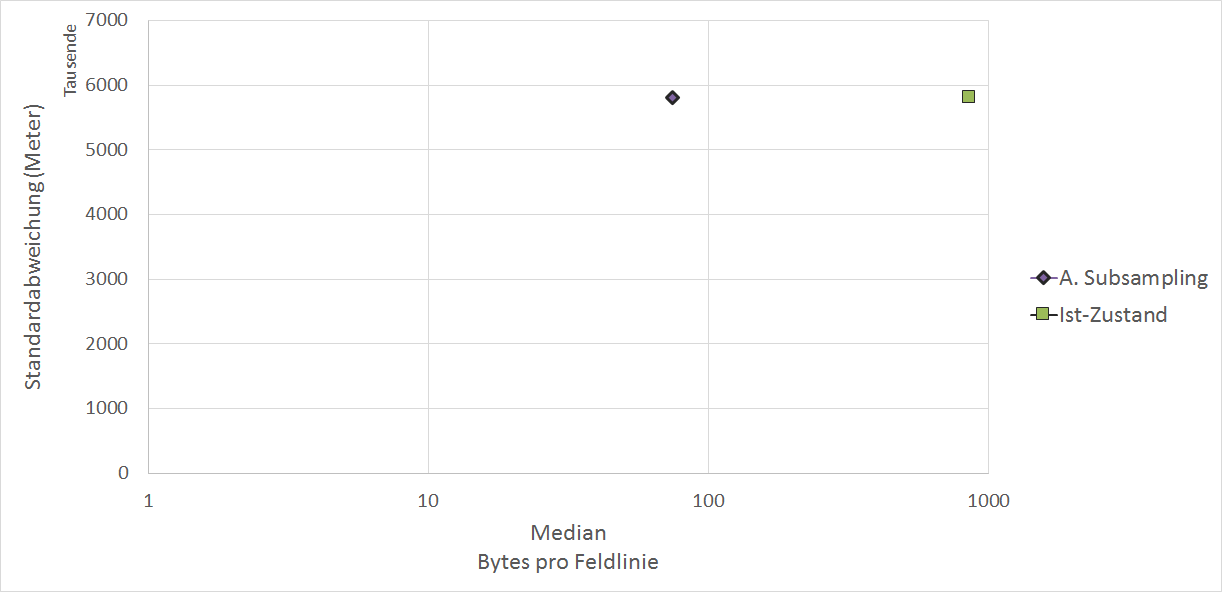
\includegraphics[width=1\textwidth,keepaspectratio]{./pictures/resultate/loesung0/loesung0_0.png}
	\caption{Vergleich des Lösungsansatzes: Adaptives Subsampling zur Ist-Kompression.}
	\label{resultate:loesung0:loesung0_0}
\end{figure}
Wie im Diagramm der Abbildung \ref{resultate:loesung0:loesung0_0} erkennbar ist, braucht dieser Lösungsansatz deutlich weniger Speicher als die Ist-Kompression zur selben Genauigkeit. Der Lösungsansatz des Adaptiven Subsamplings erreicht eine Kompressionsrate von $11.6$ gegenüber dem Ist-Zustand, indem es nur die Punkte überträgt, welche der JHelioviewers darstellt.

\begin{figure}[!htbp]
	\center
	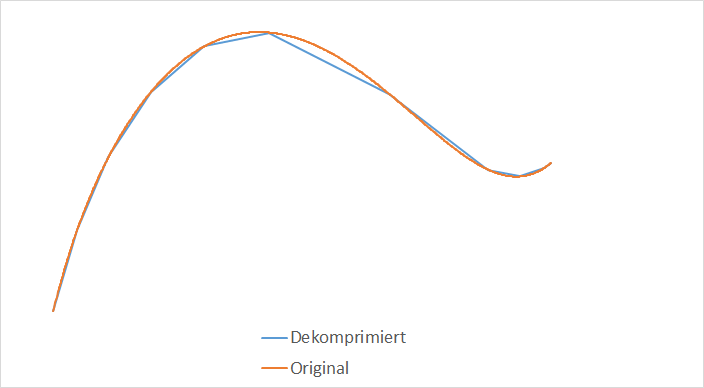
\includegraphics[width=1\textwidth,height=8cm,keepaspectratio]{./pictures/resultate/loesung0/loesung0_artefakte.png}
	\caption{Artefakte des Lösungsansatzes Adaptives Subsampling.}
	\label{resultate:loesung0:artefakte}
\end{figure}
Das Diagramm Abbildung \ref{resultate:loesung0:artefakte} zeigt die Artefakte der Kompression. Sie sind identisch mit den Artefakten der Visualisierung im Ist-Zustand. Die Artefakte sind in der JHelioviewer Visualisierung erst bei höheren Zoom-Stufen erkennbar.

Der JHelioviewer muss in der Lage sein $1000$ komprimierte Simulationen im Arbeitsspeicher abzulegen. Mit dieser Kompression werden durchschnittlich $85$ Megabyte an Arbeitsspeicher benötigt. Wenn von einer $10$ Megabit Internetverbindung ausgegangen wird, werden für das Herunterladen von $1000$ Simulationen $70$ Sekunden benötigt. Der Ist Zustand benötigt bei den selben Bedingungen $790$ Sekunden ($13$ Minuten) für die Übertragung. Mit dieser Kompression können etwa $14$ komprimierte Simulationen pro Sekunde übertragen werden. 

Ein Vorteil dieses Lösungsansatzes ist die Laufzeit Dekompression: Da keine rechenaufwändige Transformationen verwendet werden braucht dieser Lösungsansatz $19$ Millisekunden für eine Dekompression (Siehe Abschnitt \ref{anhang:performance}). Mit einem Thread ist die Testmaschine in der Lage $50$ Simulationen pro Sekunde zu dekomprimieren.

In Zukunft ist es möglich, dass im JHelioviewer deutlich mehr Punkte dargestellt werden sollen. In diesem Fall müssen entweder mehr Daten übertragen werden oder der JHelioviewer mit einer Interpolation erweitert werden.
